\scanpage{36}
\margin{35}
$\sigma$ ayant les propriétés suivantes \inserted{$\operatorname{card}\sigma\geq2$, et}

a) \deleted{il existe un} \inserted{$\sigma$} forme un arc combinatoire sur l'ens. des sommets du syst. de cordes.

b) Les $D_{i(s)}$ passant par les $s\in\sigma$ sont mutuellement \unsure{disjoints|distincts}, et passent par un même sommet (\unsure{bien sûr unique}) $\deleted{\unsure{a}}\inserted{t}$, et toute \deleted{droite}\inserted{corde} passant par $t$ est parmi les $D_{i(s)}$.

c) \deleted{Tout} Les $s\in\sigma$, (ce qui revient au $=$, \deleted{\unsure{l'enveloppe du petit triangle intercepté}}, les $s$ extrêmes) n'appartiennent pas à un arc de \deleted{spécialisation} générisation, ou ce qui revient au $=$, ne sont pas \deleted{\unsure{réunis}} \inserted{\unsure{au-dessus d'}} un sommet $S$ de $\Sigma$.

\figure{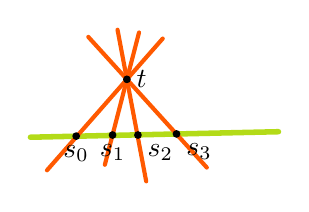
\begin{tikzpicture}[x=.7cm,y=.7cm,line cap=round]
\draw[yellow!70!green,line width=2pt] (-2,0)--(2.5,.1);
\draw[orange!70!red,line width=1.5pt] (-1.7,-.6)--(-.25,1.05)--(.4,1.79);
\draw[orange!70!red,line width=1.5pt] (-.65,-.5)--(-.25,1.05)--(-.03,1.9);
\draw[orange!70!red,line width=1.5pt] (.1,-.8)--(-.25,1.05)--(-.42,1.95);
\draw[orange!70!red,line width=1.5pt] (1.2,-.55)--(-.25,1.05)--(-.95,1.82);
\fill (-.25,1.05) circle(1.4pt) node[right]{$t$};
\fill (-1.17,0.02) circle(1.4pt) node[below]{$s_0$};
\fill (-.51,.04) circle(1.4pt) node[below]{$s_1$};
\fill (-.05,.04) circle(1.4pt) node[below right]{$s_2$};
\fill (.65,.06) circle(1.4pt) node[below right]{$s_3$};
\end{tikzpicture}}
Sous ces conditions, et supposant (comme tjrs par \unsure{ailleurs}) le système $\Sigma$ non trivial, \deleted{\unsure{alors}} il existe pour t\textsuperscript{t} $s\in\sigma$ un unique côté d'extrémités $(t,s)$, et pour $s,s'\in\sigma$ adjacents, un unique triangle de \inserted{$\Sigma$ de} sommets $t,s,s'$. La réunion de tous ces triangles s'appelle un triangle de spécialisation. Sa base, qui est l'arc géom. intercepté par l'arc combinatoire $\sigma$, est appelé un arc de spécialisation (ordinaire) \deleted{\unsure{Il y a aussi}} Tous ces arcs (fermés) sont \deleted{Il y a aussi des arcs de spécialisation} mutuellement disjoints. \deleted{exceptionnels, qui \unsure{se}}

On va aussi définir des \uline{arcs} de spécialisation exceptionnels, qui correspondent aux couloirs de $\overline\Sigma\cup D$ admettant $D$ comme mur et tels que le sommet du couloir est sommet de $\overline\Sigma$, \deleted{\unsure{L}} \inserted{et que} \deleted{\unsure{L ne rencontre aucun sommet}} l'intérieur de \deleted{un}\unsure{tel} \inserted{(la vis)} couloir le long de $L$ est un arc sur $\partial\Delta=\widetilde D$, qui est un des deux arcs extrêmes délimités par la classe d'équivalence de cordes définie par $s$.

\figure{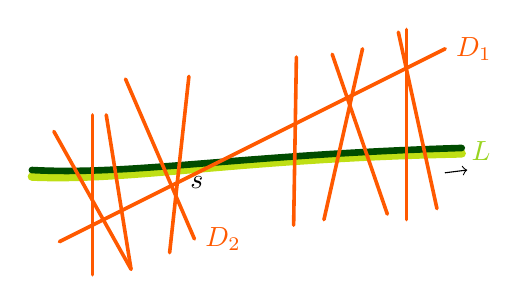
\begin{tikzpicture}[x=.7cm,y=.7cm,line cap=round]
\draw[yellow!75!green,line width=3pt] (-3.8,-.12) .. controls(-2,-.2) and(0,.22)..(4,.3);
\draw[green!30!black,line width=2.4pt] (-3.8,0)..controls(-2,-.1)and(0,.28)..(4,.4);
\draw[orange!70!red,line width=1.3pt] (-3.3,-1.3)--(3.7,2.2) node[right]{$D_1$};
\draw[orange!70!red,line width=1.3pt] (-2.1,1.65)--(-.85,-1.25) node[right]{$D_2$};
\draw[orange!70!red,line width=1.3pt] (-1.3,-1.5)--(-.95,1.7);
\draw[orange!70!red,line width=1.3pt] (-3.4,.7)--(-2,-1.8);
\draw[orange!70!red,line width=1.3pt] (-2.7,1)--(-2.7,-1.9);
\draw[orange!70!red,line width=1.3pt] (-2.45,1)--(-2,-1.8);
\draw[orange!70!red,line width=1.3pt] (.95,-1)--(1,2.05);
\draw[orange!70!red,line width=1.3pt] (1.5,-.9)--(2.2,2.2);
\draw[orange!70!red,line width=1.3pt] (1.65,2.1)--(2.65,-.8);
\draw[orange!70!red,line width=1.3pt] (3,-.9)--(3,2.55);
\draw[orange!70!red,line width=1.3pt] (3.55,-.7)--(2.85,2.5);
\node[below right] at(-1.1,.05){$s$};
\node[yellow!60!green,right]at(4,.35){$L$};\draw[->] (3.7,-.05)--(4.1,0);
\end{tikzpicture}}

\figure{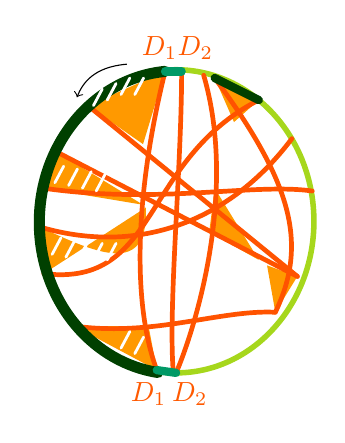
\begin{tikzpicture}[x=.7cm,y=.7cm,line cap=round,line join=round]
\draw[yellow!65!green,line width=2pt] (0,0) ellipse(2.5 and 2.75);
\fill[orange!80!yellow] (-1.6,2.1)--(-.2,2.72)--(-.6,1.4)--cycle;
\fill[orange!80!yellow] (.7,2.6)--(1.5,2.2)--(1.05,1.8)--cycle;
\fill[orange!80!yellow] (-2.4,.6)--(-.6,.3)--(-2.15,1.25)--cycle;
\fill[orange!80!yellow] (-2.48,-.1)..controls(-1.4,-.6)and(-.5,-1)..(-.55,.25)--(-2.4,-.95)--cycle;
\fill[orange!80!yellow] (.7,.6)--(1.5,-.7)--(.6,-.2)--cycle;
\fill[orange!80!yellow] (1.65,-.8)--(2.2,-1)--(1.8,-1.65)--cycle;
\fill[orange!80!yellow] (-1.85,-1.9)--(-.35,-2.7)--(-.5,-1.9)--cycle;
\draw[orange!65!red,line width=1.7pt] (-1.6,2.1)--(2.2,-1);
\draw[orange!65!red,line width=1.7pt] (-.2,2.72)..controls(-.75,.5)and(-.8,-1.5)..(-.35,-2.7);
\draw[orange!65!red,line width=1.7pt] (.1,2.72)..controls(.1,1)and(-.15,-1.6)..(-.05,-2.75);
\draw[orange!65!red,line width=1.7pt] (.5,2.65)..controls(1.1,.6)and(.4,-1.8)..(0,-2.75);
\draw[orange!65!red,line width=1.7pt] (.7,2.6)..controls(2.1,.7)and(2.4,-.4)..(1.8,-1.65);
\draw[orange!65!red,line width=1.7pt] (-2.15,1.25)--(2.2,-1);
\draw[orange!65!red,line width=1.7pt] (-2.4,.6)..controls(-.3,.3)and(1.4,.7)..(2.47,.55);
\draw[orange!65!red,line width=1.7pt] (-2.48,-.1)..controls(-.8,-.6)and(.9,-.1)..(2.1,1.5);
\draw[orange!65!red,line width=1.7pt] (-2.4,-.95)..controls(-.3,-1.2)and(-.65,1.1)..(1.5,2.2);
\draw[orange!65!red,line width=1.7pt] (-1.85,-1.9)..controls(-.4,-2.1)and(.8,-1.6)..(1.8,-1.65);
\draw[green!25!black,line width=4pt] (-.2,2.72) arc (95:262:2.5 and 2.75);
\draw[green!25!black,line width=3pt] (.7,2.6)--(1.5,2.2);
\draw[blue!40!green,line width=3pt] (-.2,2.72)--(.1,2.72);
\draw[blue!40!green,line width=3pt] (-.35,-2.7)--(0,-2.75);
\draw[->](-.9,2.85)..controls(-1.5,2.8)and(-1.7,2.5)..(-1.8,2.25);
\node[orange!70!red,above]at(-.3,2.75){$D_1$};\node[orange!70!red,above]at(.35,2.75){$D_2$};
\node[orange!70!red,below]at(-.5,-2.75){$D_1$};\node[orange!70!red,below]at(.25,-2.75){$D_2$};
\foreach \x/\y in {-1.5/2.1,-1.25/2.2,-1/2.3,-.75/2.3,-2.2/.7,-1.95/.65,-1.7/.6,-1.45/.55,-2.25/-.6,-2/-.65,-1.75/-.65,-1.5/-.7,-1.25/-.7,-1/-2.3,-.75/-2.4} {\draw[white,line width=1pt](\x,\y)--+( .16,.3);}
\end{tikzpicture}}
Ce n'est pas un arc de spécialisation ordinaire (car les \deleted{\unsure{deux}} extrémités sont dans le $=$ \deleted{deux} arc $D_1$) et on voit même que cet arc ne rencontre aucun arc de spécialisation \inserted{ordinaire} ni d'arc de générisation.
